\documentclass{article}
%encoding
%--------------------------------------
\usepackage[utf8]{inputenc}
\usepackage[T1]{fontenc}
%--------------------------------------
 
%German-specific commands
%--------------------------------------
\usepackage[ngerman]{babel}
\usepackage{csquotes}
%--------------------------------------

%Margins
%--------------------------------------
\usepackage{geometry}
 \geometry{
 a4paper,
 total={170mm,257mm},
 left=20mm,
 top=20mm,
 }
 
%Pictures
%--------------------------------------
\usepackage{graphicx}
\graphicspath{ {./Pictures/} }
\usepackage{tikz}
\usepackage{subcaption}
\usepackage{float}
\usepackage{wrapfig}
%--------------------------------------

%math
%--------------------------------------
\usepackage{amsmath}
\usepackage{amssymb}
\usepackage{amsfonts}
%--------------------------------------

%Frames
%--------------------------------------
\usepackage{framed}

%Own math commands
%--------------------------------------
\newcommand{\abs}[1]{\lvert#1\rvert}

%Colors
%--------------------------------------
\usepackage{xcolor}
\definecolor{blue-violet}{rgb}{0.54, 0.17, 0.89}
\definecolor{codegreen}{rgb}{0,0.6,0}
\definecolor{codegray}{rgb}{0.5,0.5,0.5}
\definecolor{codepurple}{rgb}{0.58,0,0.82}
\definecolor{backcolour}{rgb}{0.95,0.95,0.92}

%--------------------------------------
%\usepackage{multicol}
\usepackage{paracol}
\usepackage[shortlabels]{enumitem}

%Aufgaben
%--------------------------------------
\usepackage{amsthm}
\newtheorem{aufgabe}{Aufgabe}[section]
\newtheorem{definition}{Definition}[section]
\newtheorem{beispiel}{Beispiel}[section]
%--------------------------------------

%Listings
%--------------------------------------
\usepackage{ulem}
\usepackage{listings}
 
\lstdefinestyle{mystyle}{
    backgroundcolor=\color{backcolour},   
    commentstyle=\color{codegreen},
    keywordstyle=\color{magenta},
    numberstyle=\tiny\color{codegray},
    stringstyle=\color{codepurple},
    basicstyle=\ttfamily\footnotesize,
    breakatwhitespace=false,  
    language=Python,
    otherkeywords={repeat},       
    breaklines=true,                 
    captionpos=b,                    
    keepspaces=true,                 
    numbers=left,                    
    numbersep=5pt,                  
    showspaces=false,                
    showstringspaces=false,
    showtabs=false,                  
    tabsize=2,
}
 
\lstset{style=mystyle,moredelim=[is][\sout]{|}{|}}
%--------------------------------------



\title{Schwierige Repeat Aufgaben für Kurs 2, Woche 2}
\author{Alexandra Maximova}
\date{9. Januar 2021}

\begin{document}

\maketitle

\begin{aufgabe} \label{stern_einfach}
Schreibe ein Programm, welches einen Stern zeichnet. Du darfst die Farbe selber wählen.
\begin{figure}[H]
\centering

\includegraphics[width=0.35\linewidth]{pictures/stern1.png}
\end{figure}
\end{aufgabe}

\begin{aufgabe} \label{stern_rand}
Schreibe ein Programm, um einen Stern ohne inneres Fünfeck zu zeichnen.
\begin{figure}[H]
\centering

\includegraphics[width=0.35\linewidth]{pictures/stern2.png}
\end{figure}
\end{aufgabe}

\begin{aufgabe} \label{meander}
Mäander sind orthogonale Ornamente, die oft in der antiken griechischen und römischen Kunst vorkommen. Im antiken Griechenland sind sie als Fries in der Architektur oder als Bordüre bei Gewändern oder Keramiken zu finden.

Schreibe ein Programm, das dieses Mäander zeichnet. Die Höhe des Mäanders beträgt 100 Schildkrötenschritte. Wähle die Farbe und die Anzahl der Wiederholungen.
\begin{figure}[H]
\centering

\includegraphics[width=0.9\linewidth]{pictures/greek-meander.png}
\end{figure}
\end{aufgabe}

\begin{aufgabe} \label{proportionen}
Schreibe ein Programm, welches dieses Bild zeichnet. Beachte, dass der zentrale Stern genau zwei Mal grösser ist, als die äussere Sterne und das Bild symmetrisch ist.
\begin{figure}[H]
\centering

\includegraphics[width=0.9\linewidth]{pictures/stern-proportion-symmetrie.png}
\end{figure}
\end{aufgabe}

\begin{aufgabe} \label{quadrate}
Verbinde die Programme mit den Figuren, die sie zeichnen:
\begin{paracol}{2}
\begin{enumerate}[(1)]
\item
\begin{minipage}{\linewidth}
\lstinputlisting[language=Python]{programs/quadrate-gluecksklee.py}
\end{minipage}

\item
\begin{minipage}{\linewidth}
\lstinputlisting[language=Python]{programs/quadrate3x4.py}
\end{minipage}

\item
\begin{minipage}{\linewidth}
\lstinputlisting[language=Python]{programs/quadrate3x4-1x4.py}
\end{minipage}

\item
\begin{minipage}{\linewidth}
\lstinputlisting[language=Python]{programs/quadrate6x2.py}
\end{minipage}

\item
\begin{minipage}{\linewidth}
\lstinputlisting[language=Python]{programs/quadrate4x3.py}
\end{minipage}

\item
\begin{minipage}{\linewidth}
\lstinputlisting[language=Python]{programs/quadrate3x4-schraeg.py}
\end{minipage}
\end{enumerate}

\switchcolumn

\begin{enumerate}[(a)]
\item
\begin{minipage}{\linewidth}
\centering
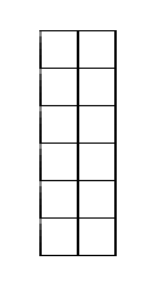
\includegraphics[width=0.5\linewidth]{pictures/quadrate6x2.png}
\end{minipage}

\item
\begin{minipage}{\linewidth}
\centering
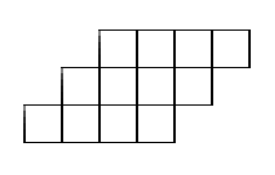
\includegraphics[width=0.9\linewidth]{pictures/quadrate3x4-schraeg.png}
\end{minipage}

\item
\begin{minipage}{\linewidth}
\centering
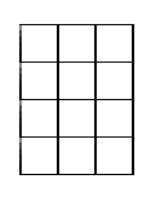
\includegraphics[width=0.6\linewidth]{pictures/quadrate4x3.png}
\end{minipage}

\item
\begin{minipage}{\linewidth}
\centering
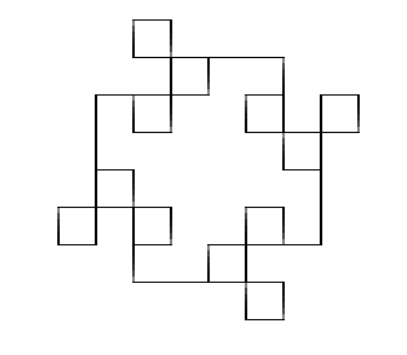
\includegraphics[width=\linewidth]{pictures/quadrate-gluecksklee.png}
\end{minipage}

\item
\begin{minipage}{\linewidth}
\vspace{10mm}
\centering
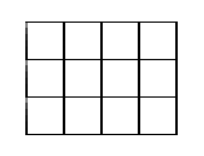
\includegraphics[width=0.7\linewidth]{pictures/quadrate3x4.png}
\vspace{10mm}
\end{minipage}

\item
\begin{minipage}{\linewidth}
\vspace{20mm}
\centering
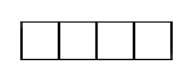
\includegraphics[width=0.7\linewidth]{pictures/quadrate3x4-1x4.png}
\vspace{20mm}
\end{minipage}
\end{enumerate}

\end{paracol}
\end{aufgabe}

\begin{aufgabe} \label{anticross-stitch-curve}
Das Endziel ist, diese Kurve zu zeichnen, ohne den Stift anzuheben, Farbe zu wechseln oder mehrmals über die gleiche Strecke zu zeichnen.
\begin{figure}[H]
\centering
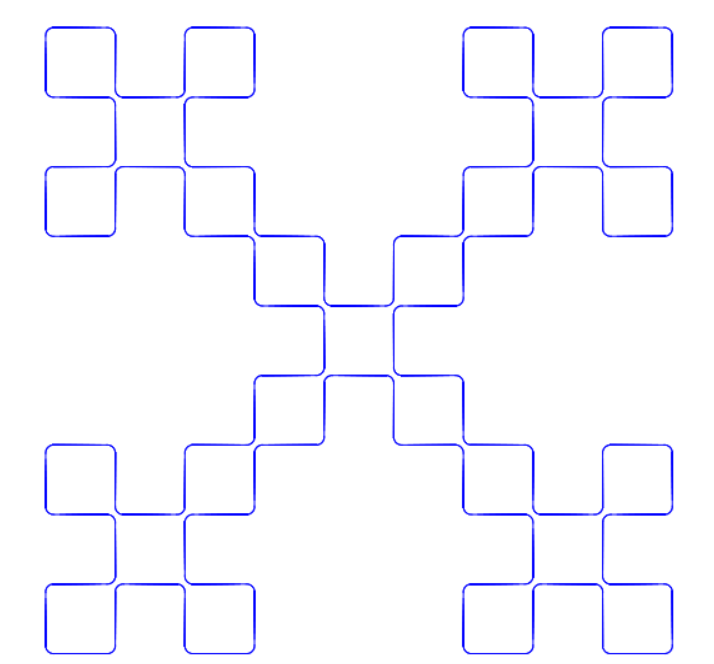
\includegraphics[width=0.6\linewidth]{pictures/anticross-stitch-curve2-round-corners.png}
\end{figure}
Schreibe zuerst ein Programm, welches diese fünf Quadrate zeichnet.
\begin{figure}[H]
\centering
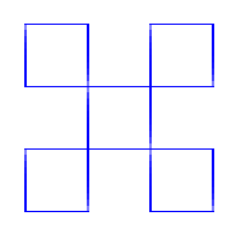
\includegraphics[width=0.3\linewidth]{pictures/anticross-stitch-curve1.png}
\end{figure}
Die runden Ecken sind optional, du kannst es auch mit normalen Ecken zeichnen. Versuche aber trotzdem die Kurve mit einer Linie zu zeichnen, ohne den Stift anzuheben oder mehrmals über die selbe Strecke zu zeichnen.

Schaffst du es, die Kurve mit den spitzen Ecken mit nur 16 Zeilen zu zeichnen (ausgenommen leere Zeilen, Kommentare, Farbenwechsel und eventuelle Drehungen und Zentrierungen am Anfang)?
\end{aufgabe}



\newpage

\section*{Beispiellösungen}


\paragraph{Aufgabe \ref{stern_einfach}}
Dieses Programm zeichnet einen Stern:
\lstinputlisting[language=Python]{programs/stern1.py}

\paragraph{Aufgabe \ref{stern_rand}}
Dieses Programm zeichnet einen Stern ohne Fünfeck:
\lstinputlisting[language=Python]{programs/stern2.py}

\paragraph{Aufgabe \ref{meander}}
Dieses Programm zeichnet einen Mäander:
\lstinputlisting[language=Python]{programs/greek-meander.py}

\paragraph{Aufgabe \ref{proportionen}}
Dieses Programm zeichnet drei Sterne:
\lstinputlisting[language=Python]{programs/stern-proportion-symmetrie.py}

\paragraph{Aufgabe \ref{quadrate}}
1d, 2e, 3f, 4a, 5c, 6b

\paragraph{Aufgabe \ref{anticross-stitch-curve}}
Eine Möglichkeit, die fünf Quadrate zu zeichnen, ist bei der unteren linken Ecke anzufangen, bis zur oberen linken Ecke entlang der Kurve zu zeichnen, und diese Zeilen vier Mal zu wiederholen.
\begin{figure}[H]
\centering
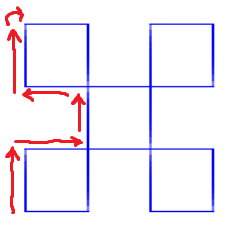
\includegraphics[width=0.3\linewidth]{pictures/anticross-stitch-curve1-expl.png}
\end{figure}
\lstinputlisting[language=Python]{programs/anticross-stitch-curve1.py}


Eine Möglichkeit, die Kurve zu zeichnen (hier mit spitzen Ecken), ist bei der unteren linken Ecke vom mittleren Quadratfünfer anzufangen, die Kurve bis zur oberen linken Ecke zu folgen, dann das Programm aus dem ersten Teil benutzen, um einen Quadratfünfer zu zeichnen. Um die ganze Kurve zu zeichnen, muss man das vier Mal wiederholen.
\begin{figure}[H]
\centering
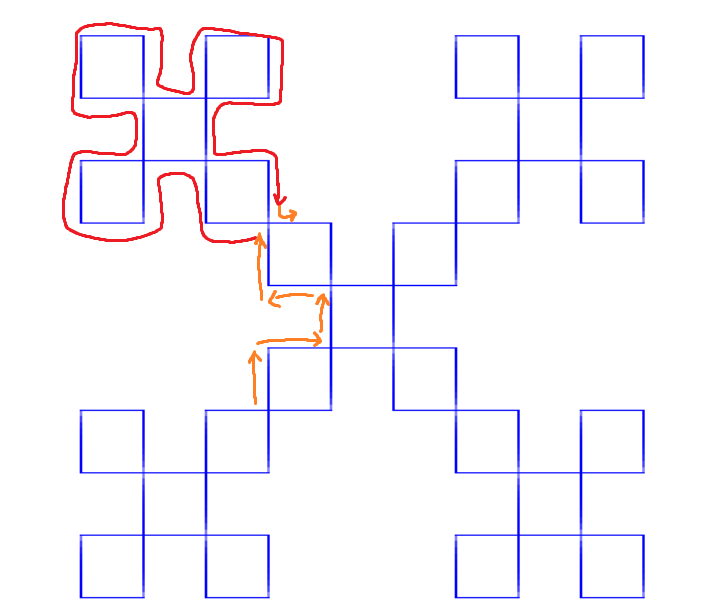
\includegraphics[width=0.6\linewidth]{pictures/anticross-stitch-curve2-expl.png}
\end{figure}
\lstinputlisting[language=Python]{programs/anticross-stitch-curve2.py}

Die Kurve mit den spitzen Ecken lässt sich auch kürzer Zeichnen. Dafür müssen wir aber gezeichnete Linien kreuzen, das würde in der Version mit den runden Ecken nicht funktionieren.
\begin{figure}[H]
\centering
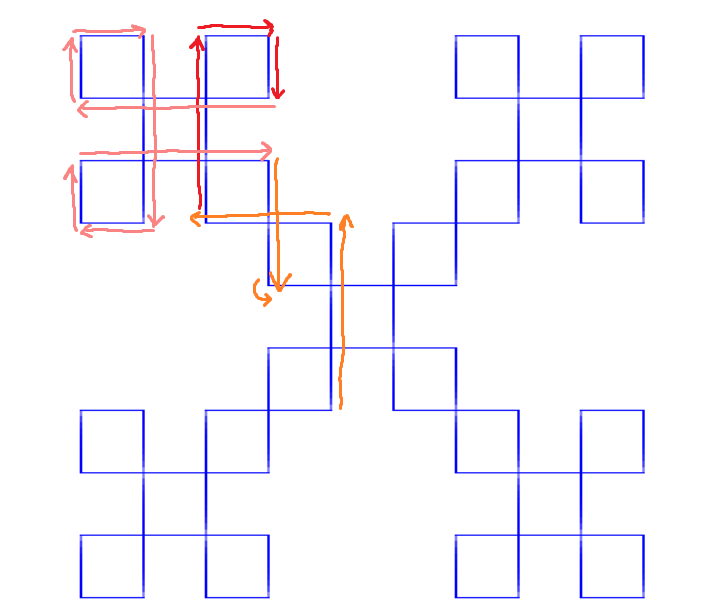
\includegraphics[width=0.6\linewidth]{pictures/anticross-stitch-curve2-intersect-expl.png}
\end{figure}
\lstinputlisting[language=Python]{programs/anticross-stitch-curve2-intersect.py}

\end{document}